The simply supported beam has a pin at the left and a roller at the right. Each support prevents transverse displacement and permits rotation. The roller also permits axial motion.

\begin{figure}[H]
\centering
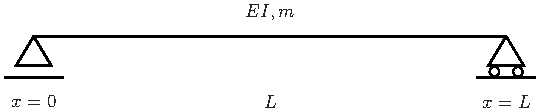
\includegraphics[width=0.65\linewidth]{figures/generated/solutions/C4_support.pdf}
\caption{Simply supported beam with constant bending stiffness and mass per unit length.}
\end{figure}

The notes give zero transverse displacement and zero bending moment at each end (course notes, flexural vibration, PDF pp. 193--195). The shear force is a support reaction and is not prescribed to be zero. Since \(M=EIw_{xx}\), the four conditions are
\[
w(0,t)=w(L,t)=0,\qquad M(0,t)=M(L,t)=0
\quad\Longrightarrow\quad W(0)=W(L)=W''(0)=W''(L)=0.
\]
Write the separated motion as \(w(x,t)=W(x)e^{-i\omega t}\), with
\[
W=C_1\sin\gamma x+C_2\cos\gamma x+C_3\sinh\gamma x+C_4\cosh\gamma x.
\]
The conditions at zero give \(C_2+C_4=0\) and \(-C_2+C_4=0\). Thus \(C_2=C_4=0\). At \(x=L\), with \(z=\gamma L\), the two remaining equations are
\[
C_1\sin z+C_3\sinh z=0,\qquad
-C_1\sin z+C_3\sinh z=0.
\]
The zero vector of constants gives the trivial motion. Nonzero motion requires the determinant \(2\sin z\sinh z\) to vanish. The positive roots are \(z_j=j\pi\), \(j=1,2,\ldots\). The zero root is excluded because it produces only the trivial static shape under these boundary conditions. Since \(\sinh z_j\ne0\), \(C_3=0\), and choosing \(C_1=1\) gives
\[
\gamma_j=\frac{j\pi}{L},\quad W_j(x)=\sin\frac{j\pi x}{L},\quad
\qquad j=1,2,\ldots.
\]
The flexural dispersion relation $\omega=a^2\gamma^2$ then converts each spatial root to a frequency. With $a=(EI/m)^{1/4}$, this gives
\[
\omega_j=\left(\frac{j\pi}{L}\right)^2\sqrt{\frac{EI}{m}},\qquad f_j=\frac{\omega_j}{2\pi}.
\]
Thus the amplitude-normalized modes satisfy
\[
\int_0^L W_pW_q\,dx=\frac L2\delta_{pq}.
\]
For unit integral, use \(\phi_j=\sqrt{2/L}W_j\), so \(\int_0^L\phi_p\phi_q\,dx=\delta_{pq}\). Mass normalization instead uses \(\sqrt{2/(mL)}W_j\).
